
\documentclass[tikz, border=1mm]{standalone}

\usepackage{amsmath}

\usetikzlibrary{calc,angles,quotes}

\begin{document}
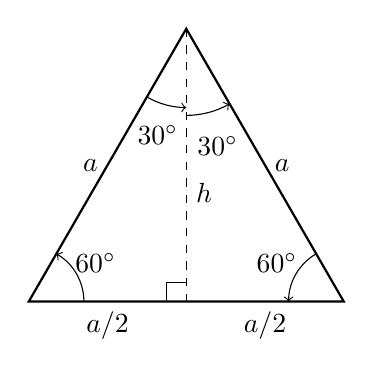
\begin{tikzpicture}[scale=4.0]

	% triangle 3 - 4 - 5
	\def\a{60}

	% points
	\coordinate (A) at (0,0);
	\coordinate (B) at ({cos(\a)},{sin(\a)});
	\coordinate (C) at ({2*cos(\a)},0);

	% feet of altitude from B to AC
	\coordinate (D) at ({cos(\a)},0);

	% triangle sides
	\draw[thick] (A) -- (B) -- (C) -- cycle;

	% altitude
	\draw[dashed] (B) -- (D);

	% side labels
	\node[left]  at ($(A)!0.5!(B)$) {$a$};
	\node[right] at ($(B)!0.5!(C)$) {$a$};

	% segment labels on altitude projection
	\node[below] at ($(A)!0.5!(D)$) {$a/2$};
	\node[below] at ($(D)!0.5!(C)$) {$a/2$};

	% height label
	\node[right] at ($(B)!0.6!(D)$) {$h$};

	% angle labels
	\pic["$60^\circ$", draw, ->, angle eccentricity=1.4, angle radius=0.7cm]
		{angle = C--A--B};
	\pic["$30^\circ$", draw, ->, angle eccentricity=1.4, angle radius=1.0cm]
		{angle = A--B--D};
	\pic["$60^\circ$", draw, ->, angle eccentricity=1.4, angle radius=0.7cm]
		{angle = B--C--A};
	\pic["$30^\circ$", draw, ->, angle eccentricity=1.4, angle radius=1.1cm]
		{angle = D--B--C};

	% right angle marker
	\pic [draw, angle radius=7pt, angle eccentricity=1]
	{right angle = A--D--B};

\end{tikzpicture}
\end{document}
